\documentclass[1p]{elsarticle_modified}
%\bibliographystyle{elsarticle-num}

%\usepackage[colorlinks]{hyperref}
%\usepackage{abbrmath_seonhwa} %\Abb, \Ascr, \Acal ,\Abf, \Afrak
\usepackage{amsfonts}
\usepackage{amssymb}
\usepackage{amsmath}
\usepackage{amsthm}
\usepackage{scalefnt}
\usepackage{amsbsy}
\usepackage{kotex}
\usepackage{caption}
\usepackage{subfig}
\usepackage{color}
\usepackage{graphicx}
\usepackage{xcolor} %% white, black, red, green, blue, cyan, magenta, yellow
\usepackage{float}
\usepackage{setspace}
\usepackage{hyperref}

\usepackage{tikz}
\usetikzlibrary{arrows}

\usepackage{multirow}
\usepackage{array} % fixed length table
\usepackage{hhline}

%%%%%%%%%%%%%%%%%%%%%
\makeatletter
\renewcommand*\env@matrix[1][\arraystretch]{%
	\edef\arraystretch{#1}%
	\hskip -\arraycolsep
	\let\@ifnextchar\new@ifnextchar
	\array{*\c@MaxMatrixCols c}}
\makeatother %https://tex.stackexchange.com/questions/14071/how-can-i-increase-the-line-spacing-in-a-matrix
%%%%%%%%%%%%%%%

\usepackage[normalem]{ulem}

\newcommand{\msout}[1]{\ifmmode\text{\sout{\ensuremath{#1}}}\else\sout{#1}\fi}
%SOURCE: \msout is \stkout macro in https://tex.stackexchange.com/questions/20609/strikeout-in-math-mode

\newcommand{\cancel}[1]{
	\ifmmode
	{\color{red}\msout{#1}}
	\else
	{\color{red}\sout{#1}}
	\fi
}

\newcommand{\add}[1]{
	{\color{blue}\uwave{#1}}
}

\newcommand{\replace}[2]{
	\ifmmode
	{\color{red}\msout{#1}}{\color{blue}\uwave{#2}}
	\else
	{\color{red}\sout{#1}}{\color{blue}\uwave{#2}}
	\fi
}

\newcommand{\Sol}{\mathcal{S}} %segment
\newcommand{\D}{D} %diagram
\newcommand{\A}{\mathcal{A}} %arc


%%%%%%%%%%%%%%%%%%%%%%%%%%%%%5 test

\def\sl{\operatorname{\textup{SL}}(2,\Cbb)}
\def\psl{\operatorname{\textup{PSL}}(2,\Cbb)}
\def\quan{\mkern 1mu \triangleright \mkern 1mu}

\theoremstyle{definition}
\newtheorem{thm}{Theorem}[section]
\newtheorem{prop}[thm]{Proposition}
\newtheorem{lem}[thm]{Lemma}
\newtheorem{ques}[thm]{Question}
\newtheorem{cor}[thm]{Corollary}
\newtheorem{defn}[thm]{Definition}
\newtheorem{exam}[thm]{Example}
\newtheorem{rmk}[thm]{Remark}
\newtheorem{alg}[thm]{Algorithm}

\newcommand{\I}{\sqrt{-1}}
\begin{document}

%\begin{frontmatter}
%
%\title{Boundary parabolic representations of knots up to 8 crossings}
%
%%% Group authors per affiliation:
%\author{Yunhi Cho} 
%\address{Department of Mathematics, University of Seoul, Seoul, Korea}
%\ead{yhcho@uos.ac.kr}
%
%
%\author{Seonhwa Kim} %\fnref{s_kim}}
%\address{Center for Geometry and Physics, Institute for Basic Science, Pohang, 37673, Korea}
%\ead{ryeona17@ibs.re.kr}
%
%\author{Hyuk Kim}
%\address{Department of Mathematical Sciences, Seoul National University, Seoul 08826, Korea}
%\ead{hyukkim@snu.ac.kr}
%
%\author{Seokbeom Yoon}
%\address{Department of Mathematical Sciences, Seoul National University, Seoul, 08826,  Korea}
%\ead{sbyoon15@snu.ac.kr}
%
%\begin{abstract}
%We find all boundary parabolic representation of knots up to 8 crossings.
%
%\end{abstract}
%\begin{keyword}
%    \MSC[2010] 57M25 
%\end{keyword}
%
%\end{frontmatter}

%\linenumbers
%\tableofcontents
%
\newcommand\colored[1]{\textcolor{white}{\rule[-0.35ex]{0.8em}{1.4ex}}\kern-0.8em\color{red} #1}%
%\newcommand\colored[1]{\textcolor{white}{ #1}\kern-2.17ex	\textcolor{white}{ #1}\kern-1.81ex	\textcolor{white}{ #1}\kern-2.15ex\color{red}#1	}

{\Large $\underline{12a_{0222}~(K12a_{0222})}$}

\setlength{\tabcolsep}{10pt}
\renewcommand{\arraystretch}{1.6}
\vspace{1cm}\begin{tabular}{m{100pt}>{\centering\arraybackslash}m{274pt}}
\multirow{5}{120pt}{
	\centering
	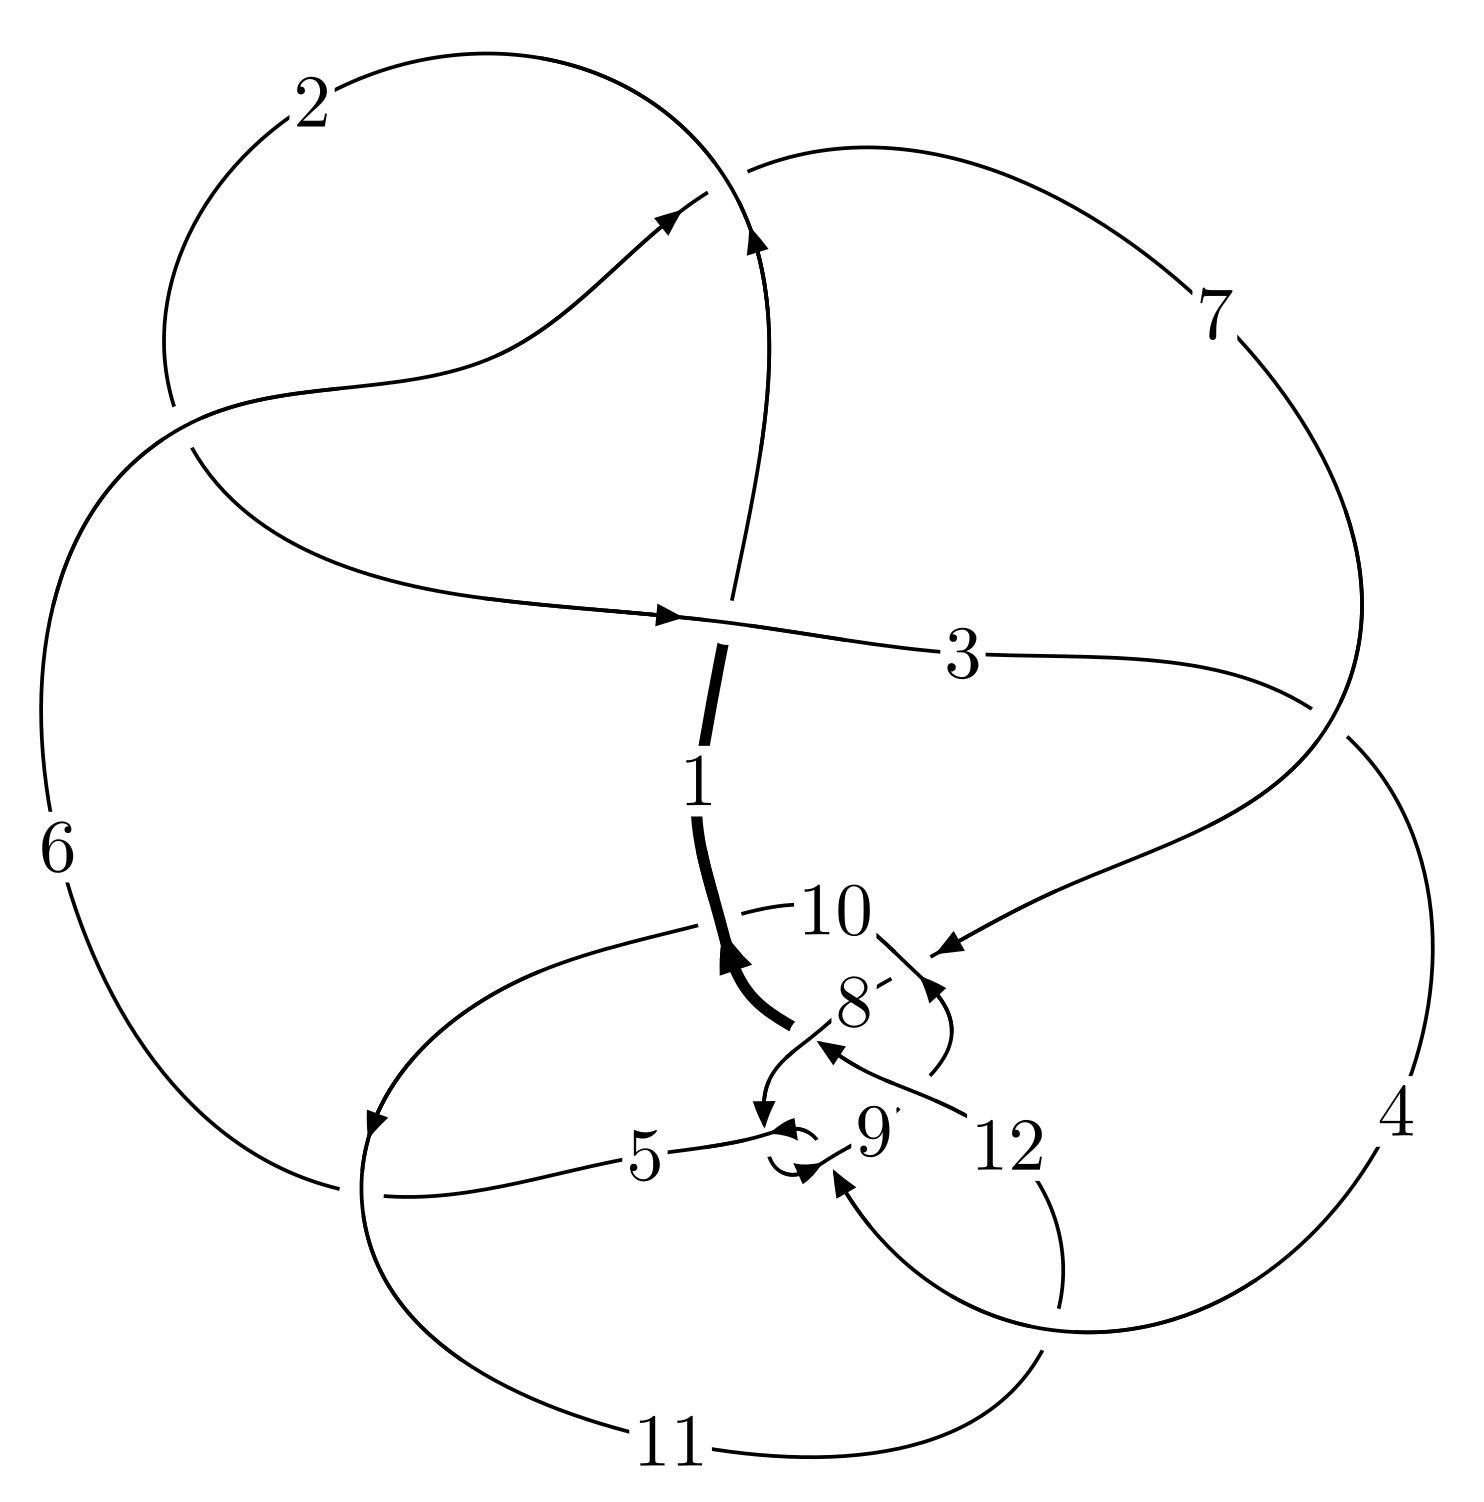
\includegraphics[width=112pt]{../../../GIT/diagram.site/Diagrams/png/1023_12a_0222.png}\\
\ \ \ A knot diagram\footnotemark}&
\allowdisplaybreaks
\textbf{Linearized knot diagam} \\
\cline{2-2}
 &
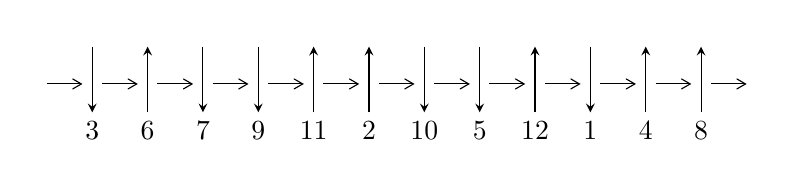
\begin{tikzpicture}[x=20pt, y=17pt]
	% nodes
	\node (C0) at (0, 0) {};
	\node (C1) at (1, 0) {};
	\node (C1U) at (1, +1) {};
	\node (C1D) at (1, -1) {3};

	\node (C2) at (2, 0) {};
	\node (C2U) at (2, +1) {};
	\node (C2D) at (2, -1) {6};

	\node (C3) at (3, 0) {};
	\node (C3U) at (3, +1) {};
	\node (C3D) at (3, -1) {7};

	\node (C4) at (4, 0) {};
	\node (C4U) at (4, +1) {};
	\node (C4D) at (4, -1) {9};

	\node (C5) at (5, 0) {};
	\node (C5U) at (5, +1) {};
	\node (C5D) at (5, -1) {11};

	\node (C6) at (6, 0) {};
	\node (C6U) at (6, +1) {};
	\node (C6D) at (6, -1) {2};

	\node (C7) at (7, 0) {};
	\node (C7U) at (7, +1) {};
	\node (C7D) at (7, -1) {10};

	\node (C8) at (8, 0) {};
	\node (C8U) at (8, +1) {};
	\node (C8D) at (8, -1) {5};

	\node (C9) at (9, 0) {};
	\node (C9U) at (9, +1) {};
	\node (C9D) at (9, -1) {12};

	\node (C10) at (10, 0) {};
	\node (C10U) at (10, +1) {};
	\node (C10D) at (10, -1) {1};

	\node (C11) at (11, 0) {};
	\node (C11U) at (11, +1) {};
	\node (C11D) at (11, -1) {4};

	\node (C12) at (12, 0) {};
	\node (C12U) at (12, +1) {};
	\node (C12D) at (12, -1) {8};
	\node (C13) at (13, 0) {};

	% arrows
	\draw[->,>={angle 60}]
	(C0) edge (C1) (C1) edge (C2) (C2) edge (C3) (C3) edge (C4) (C4) edge (C5) (C5) edge (C6) (C6) edge (C7) (C7) edge (C8) (C8) edge (C9) (C9) edge (C10) (C10) edge (C11) (C11) edge (C12) (C12) edge (C13) ;	\draw[->,>=stealth]
	(C1U) edge (C1D) (C2D) edge (C2U) (C3U) edge (C3D) (C4U) edge (C4D) (C5D) edge (C5U) (C6D) edge (C6U) (C7U) edge (C7D) (C8U) edge (C8D) (C9D) edge (C9U) (C10U) edge (C10D) (C11D) edge (C11U) (C12D) edge (C12U) ;
	\end{tikzpicture} \\
\hhline{~~} \\& 
\textbf{Solving Sequence} \\ \cline{2-2} 
 &
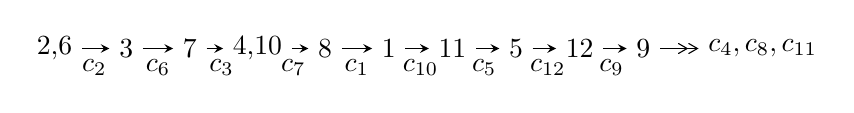
\begin{tikzpicture}[x=23pt, y=7pt]
	% node
	\node (A0) at (-1/8, 0) {2,6};
	\node (A1) at (1, 0) {3};
	\node (A2) at (2, 0) {7};
	\node (A3) at (49/16, 0) {4,10};
	\node (A4) at (33/8, 0) {8};
	\node (A5) at (41/8, 0) {1};
	\node (A6) at (49/8, 0) {11};
	\node (A7) at (57/8, 0) {5};
	\node (A8) at (65/8, 0) {12};
	\node (A9) at (73/8, 0) {9};
	\node (C1) at (1/2, -1) {$c_{2}$};
	\node (C2) at (3/2, -1) {$c_{6}$};
	\node (C3) at (5/2, -1) {$c_{3}$};
	\node (C4) at (29/8, -1) {$c_{7}$};
	\node (C5) at (37/8, -1) {$c_{1}$};
	\node (C6) at (45/8, -1) {$c_{10}$};
	\node (C7) at (53/8, -1) {$c_{5}$};
	\node (C8) at (61/8, -1) {$c_{12}$};
	\node (C9) at (69/8, -1) {$c_{9}$};
	\node (A10) at (11, 0) {$c_{4},c_{8},c_{11}$};

	% edge
	\draw[->,>=stealth]	
	(A0) edge (A1) (A1) edge (A2) (A2) edge (A3) (A3) edge (A4) (A4) edge (A5) (A5) edge (A6) (A6) edge (A7) (A7) edge (A8) (A8) edge (A9) ;
	\draw[->>,>={angle 60}]	
	(A9) edge (A10);
\end{tikzpicture} \\ 

\end{tabular} \\

\footnotetext{
The image of knot diagram is generated by the software ``\textbf{Draw programme}" developed by Andrew Bartholomew(\url{http://www.layer8.co.uk/maths/draw/index.htm\#Running-draw}), where we modified some parts for our purpose(\url{https://github.com/CATsTAILs/LinksPainter}).
}\phantom \\ \newline 
\centering \textbf{Ideals for irreducible components\footnotemark of $X_{\text{par}}$} 
 
\begin{align*}
I^u_{1}&=\langle 
2 u^{36}+u^{35}+\cdots+b-9,\;3 u^{36}-3 u^{35}+\cdots+a+1,\;u^{37}-2 u^{36}+\cdots+2 u-1\rangle \\
\\
\end{align*}
\raggedright * 1 irreducible components of $\dim_{\mathbb{C}}=0$, with total 37 representations.\\
\footnotetext{All coefficients of polynomials are rational numbers. But the coefficients are sometimes approximated in decimal forms when there is not enough margin.}
\newpage
\renewcommand{\arraystretch}{1}
\centering \section*{I. $I^u_{1}= \langle 2 u^{36}+u^{35}+\cdots+b-9,\;3 u^{36}-3 u^{35}+\cdots+a+1,\;u^{37}-2 u^{36}+\cdots+2 u-1 \rangle$}
\flushleft \textbf{(i) Arc colorings}\\
\begin{tabular}{m{7pt} m{180pt} m{7pt} m{180pt} }
\flushright $a_{2}=$&$\begin{pmatrix}1\\0\end{pmatrix}$ \\
\flushright $a_{6}=$&$\begin{pmatrix}0\\u\end{pmatrix}$ \\
\flushright $a_{3}=$&$\begin{pmatrix}1\\- u^2\end{pmatrix}$ \\
\flushright $a_{7}=$&$\begin{pmatrix}u\\u\end{pmatrix}$ \\
\flushright $a_{4}=$&$\begin{pmatrix}u^4+u^2+1\\u^4\end{pmatrix}$ \\
\flushright $a_{10}=$&$\begin{pmatrix}-3 u^{36}+3 u^{35}+\cdots+5 u-1\\-2 u^{36}- u^{35}+\cdots+u+9\end{pmatrix}$ \\
\flushright $a_{8}=$&$\begin{pmatrix}-4 u^{35}+10 u^{34}+\cdots-11 u+11\\-6 u^{36}+17 u^{35}+\cdots+18 u-12\end{pmatrix}$ \\
\flushright $a_{1}=$&$\begin{pmatrix}u^2+1\\- u^4\end{pmatrix}$ \\
\flushright $a_{11}=$&$\begin{pmatrix}6 u^{36}-10 u^{35}+\cdots-12 u+1\\5 u^{36}-14 u^{35}+\cdots-14 u+15\end{pmatrix}$ \\
\flushright $a_{5}=$&$\begin{pmatrix}-3 u^{36}+2 u^{35}+\cdots+9 u+1\\11 u^{36}-15 u^{35}+\cdots-6 u-8\end{pmatrix}$ \\
\flushright $a_{12}=$&$\begin{pmatrix}2 u^{36}-3 u^{35}+\cdots-2 u+1\\3 u^{36}-7 u^{35}+\cdots-6 u+10\end{pmatrix}$ \\
\flushright $a_{9}=$&$\begin{pmatrix}2 u^{36}- u^{35}+\cdots+u-15\\5 u^{36}-12 u^{35}+\cdots-11 u+1\end{pmatrix}$\\&\end{tabular}
\flushleft \textbf{(ii) Obstruction class $= 1$}\\~\\
\flushleft \textbf{(iii) Cusp Shapes $= 50 u^{36}-53 u^{35}+513 u^{34}-472 u^{33}+2604 u^{32}-2103 u^{31}+8527 u^{30}-6002 u^{29}+19933 u^{28}-12090 u^{27}+34843 u^{26}-17999 u^{25}+46330 u^{24}-20392 u^{23}+46429 u^{22}-18028 u^{21}+33354 u^{20}-12865 u^{19}+14474 u^{18}-7621 u^{17}+482 u^{16}-3677 u^{15}-3764 u^{14}-1370 u^{13}-1746 u^{12}-705 u^{11}+628 u^{10}-954 u^9+992 u^8-1056 u^7+361 u^6-706 u^5-43 u^4-276 u^3-89 u^2-49 u-37$}\\~\\
\newpage\renewcommand{\arraystretch}{1}
\flushleft \textbf{(iv) u-Polynomials at the component}\newline \\
\begin{tabular}{m{50pt}|m{274pt}}
Crossings & \hspace{64pt}u-Polynomials at each crossing \\
\hline $$\begin{aligned}c_{1}\end{aligned}$$&$\begin{aligned}
&u^{37}-20 u^{36}+\cdots-10 u+1
\end{aligned}$\\
\hline $$\begin{aligned}c_{2}\end{aligned}$$&$\begin{aligned}
&u^{37}-2 u^{36}+\cdots+2 u-1
\end{aligned}$\\
\hline $$\begin{aligned}c_{3}\end{aligned}$$&$\begin{aligned}
&u^{37}+2 u^{36}+\cdots+8 u-1
\end{aligned}$\\
\hline $$\begin{aligned}c_{4}\end{aligned}$$&$\begin{aligned}
&u^{37}+u^{36}+\cdots- u-1
\end{aligned}$\\
\hline $$\begin{aligned}c_{5}\end{aligned}$$&$\begin{aligned}
&u^{37}-7 u^{35}+\cdots-2 u-1
\end{aligned}$\\
\hline $$\begin{aligned}c_{6}\end{aligned}$$&$\begin{aligned}
&u^{37}+2 u^{36}+\cdots+2 u+1
\end{aligned}$\\
\hline $$\begin{aligned}c_{7}\end{aligned}$$&$\begin{aligned}
&u^{37}-3 u^{36}+\cdots-7 u-1
\end{aligned}$\\
\hline $$\begin{aligned}c_{8}\end{aligned}$$&$\begin{aligned}
&u^{37}- u^{36}+\cdots- u+1
\end{aligned}$\\
\hline $$\begin{aligned}c_{9}\end{aligned}$$&$\begin{aligned}
&u^{37}+20 u^{36}+\cdots+23 u+1
\end{aligned}$\\
\hline $$\begin{aligned}c_{10}\end{aligned}$$&$\begin{aligned}
&u^{37}-17 u^{36}+\cdots+23 u-1
\end{aligned}$\\
\hline $$\begin{aligned}c_{11}\end{aligned}$$&$\begin{aligned}
&u^{37}-4 u^{36}+\cdots-2 u+1
\end{aligned}$\\
\hline $$\begin{aligned}c_{12}\end{aligned}$$&$\begin{aligned}
&u^{37}+7 u^{36}+\cdots+3 u-1
\end{aligned}$\\
\hline
\end{tabular}\\~\\
\newpage\renewcommand{\arraystretch}{1}
\flushleft \textbf{(v) Riley Polynomials at the component}\newline \\
\begin{tabular}{m{50pt}|m{274pt}}
Crossings & \hspace{64pt}Riley Polynomials at each crossing \\
\hline $$\begin{aligned}c_{1}\end{aligned}$$&$\begin{aligned}
&y^{37}+4 y^{36}+\cdots-10 y-1
\end{aligned}$\\
\hline $$\begin{aligned}c_{2},c_{6}\end{aligned}$$&$\begin{aligned}
&y^{37}+20 y^{36}+\cdots-10 y-1
\end{aligned}$\\
\hline $$\begin{aligned}c_{3}\end{aligned}$$&$\begin{aligned}
&y^{37}-6 y^{36}+\cdots+8 y-1
\end{aligned}$\\
\hline $$\begin{aligned}c_{4},c_{8}\end{aligned}$$&$\begin{aligned}
&y^{37}+21 y^{36}+\cdots-29 y-1
\end{aligned}$\\
\hline $$\begin{aligned}c_{5}\end{aligned}$$&$\begin{aligned}
&y^{37}-14 y^{36}+\cdots-12 y-1
\end{aligned}$\\
\hline $$\begin{aligned}c_{7}\end{aligned}$$&$\begin{aligned}
&y^{37}-17 y^{36}+\cdots+17 y-1
\end{aligned}$\\
\hline $$\begin{aligned}c_{9}\end{aligned}$$&$\begin{aligned}
&y^{37}+4 y^{36}+\cdots+13 y-1
\end{aligned}$\\
\hline $$\begin{aligned}c_{10}\end{aligned}$$&$\begin{aligned}
&y^{37}+7 y^{36}+\cdots+35 y-1
\end{aligned}$\\
\hline $$\begin{aligned}c_{11}\end{aligned}$$&$\begin{aligned}
&y^{37}+4 y^{36}+\cdots+24 y-1
\end{aligned}$\\
\hline $$\begin{aligned}c_{12}\end{aligned}$$&$\begin{aligned}
&y^{37}-17 y^{36}+\cdots+17 y-1
\end{aligned}$\\
\hline
\end{tabular}\\~\\
\newpage\flushleft \textbf{(vi) Complex Volumes and Cusp Shapes}
$$\begin{array}{c|c|c}  
\text{Solutions to }I^u_{1}& \I (\text{vol} + \sqrt{-1}CS) & \text{Cusp shape}\\
 \hline 
\begin{aligned}
u &= -0.149884 + 0.975736 I \\
a &= -0.898991 + 0.581003 I \\
b &= -1.59695 + 0.70098 I\end{aligned}
 & -1.70560 + 1.29082 I & -4.10550 - 4.13500 I \\ \hline\begin{aligned}
u &= -0.149884 - 0.975736 I \\
a &= -0.898991 - 0.581003 I \\
b &= -1.59695 - 0.70098 I\end{aligned}
 & -1.70560 - 1.29082 I & -4.10550 + 4.13500 I \\ \hline\begin{aligned}
u &= -0.600365 + 0.704581 I \\
a &= \phantom{-}0.757124 + 0.641967 I \\
b &= -0.204265 + 0.747533 I\end{aligned}
 & \phantom{-}0.834960 + 0.285553 I & -0.434596 + 0.220919 I \\ \hline\begin{aligned}
u &= -0.600365 - 0.704581 I \\
a &= \phantom{-}0.757124 - 0.641967 I \\
b &= -0.204265 - 0.747533 I\end{aligned}
 & \phantom{-}0.834960 - 0.285553 I & -0.434596 - 0.220919 I \\ \hline\begin{aligned}
u &= -0.479565 + 0.990246 I \\
a &= \phantom{-}0.864069 + 0.151474 I \\
b &= -0.0946240 + 0.0662065 I\end{aligned}
 & -0.363148 - 0.677922 I & \phantom{-}0.56726 + 2.15135 I \\ \hline\begin{aligned}
u &= -0.479565 - 0.990246 I \\
a &= \phantom{-}0.864069 - 0.151474 I \\
b &= -0.0946240 - 0.0662065 I\end{aligned}
 & -0.363148 + 0.677922 I & \phantom{-}0.56726 - 2.15135 I \\ \hline\begin{aligned}
u &= -0.532442 + 0.982690 I \\
a &= -0.780782 - 0.630467 I \\
b &= -0.290116 - 1.327480 I\end{aligned}
 & -0.06388 - 4.77621 I & -1.68090 + 5.53681 I \\ \hline\begin{aligned}
u &= -0.532442 - 0.982690 I \\
a &= -0.780782 + 0.630467 I \\
b &= -0.290116 + 1.327480 I\end{aligned}
 & -0.06388 + 4.77621 I & -1.68090 - 5.53681 I \\ \hline\begin{aligned}
u &= -0.204733 + 0.857295 I \\
a &= -1.38015 + 0.70474 I \\
b &= \phantom{-}0.0824504 + 0.0328733 I\end{aligned}
 & -1.37034 - 3.02368 I & -8.36272 + 7.29707 I \\ \hline\begin{aligned}
u &= -0.204733 - 0.857295 I \\
a &= -1.38015 - 0.70474 I \\
b &= \phantom{-}0.0824504 - 0.0328733 I\end{aligned}
 & -1.37034 + 3.02368 I & -8.36272 - 7.29707 I\\
 \hline 
 \end{array}$$\newpage$$\begin{array}{c|c|c}  
\text{Solutions to }I^u_{1}& \I (\text{vol} + \sqrt{-1}CS) & \text{Cusp shape}\\
 \hline 
\begin{aligned}
u &= \phantom{-}0.459092 + 1.035940 I \\
a &= \phantom{-}0.59291 + 1.57136 I \\
b &= -0.33683 + 2.07268 I\end{aligned}
 & \phantom{-}2.24562 - 1.84888 I & \phantom{-}1.43556 + 1.62892 I \\ \hline\begin{aligned}
u &= \phantom{-}0.459092 - 1.035940 I \\
a &= \phantom{-}0.59291 - 1.57136 I \\
b &= -0.33683 - 2.07268 I\end{aligned}
 & \phantom{-}2.24562 + 1.84888 I & \phantom{-}1.43556 - 1.62892 I \\ \hline\begin{aligned}
u &= \phantom{-}0.477509 + 1.033510 I \\
a &= -1.05702 + 2.06127 I \\
b &= -0.71022 + 2.96225 I\end{aligned}
 & \phantom{-}2.36710 + 8.22059 I & \phantom{-}0.94025 - 9.93315 I \\ \hline\begin{aligned}
u &= \phantom{-}0.477509 - 1.033510 I \\
a &= -1.05702 - 2.06127 I \\
b &= -0.71022 - 2.96225 I\end{aligned}
 & \phantom{-}2.36710 - 8.22059 I & \phantom{-}0.94025 + 9.93315 I \\ \hline\begin{aligned}
u &= \phantom{-}0.834958\phantom{ +0.000000I} \\
a &= -2.24679\phantom{ +0.000000I} \\
b &= \phantom{-}0.265283\phantom{ +0.000000I}\end{aligned}
 & -3.19671\phantom{ +0.000000I} & \phantom{-}32.4830\phantom{ +0.000000I} \\ \hline\begin{aligned}
u &= \phantom{-}0.325483 + 1.152650 I \\
a &= \phantom{-}0.15406 - 1.63598 I \\
b &= \phantom{-}0.69492 - 2.01501 I\end{aligned}
 & -4.68461 - 1.11526 I & -3.13705 + 0.65063 I \\ \hline\begin{aligned}
u &= \phantom{-}0.325483 - 1.152650 I \\
a &= \phantom{-}0.15406 + 1.63598 I \\
b &= \phantom{-}0.69492 + 2.01501 I\end{aligned}
 & -4.68461 + 1.11526 I & -3.13705 - 0.65063 I \\ \hline\begin{aligned}
u &= -0.500299 + 0.608166 I \\
a &= -0.471582 - 0.257960 I \\
b &= -0.12074 - 1.48951 I\end{aligned}
 & \phantom{-}0.79654 - 3.35515 I & \phantom{-}4.80142 + 6.29346 I \\ \hline\begin{aligned}
u &= -0.500299 - 0.608166 I \\
a &= -0.471582 + 0.257960 I \\
b &= -0.12074 + 1.48951 I\end{aligned}
 & \phantom{-}0.79654 + 3.35515 I & \phantom{-}4.80142 - 6.29346 I \\ \hline\begin{aligned}
u &= -0.743965 + 0.168516 I \\
a &= -1.330750 + 0.223235 I \\
b &= -0.105331 + 0.292541 I\end{aligned}
 & \phantom{-}2.40521 + 5.56732 I & \phantom{-}3.26355 - 5.71144 I\\
 \hline 
 \end{array}$$\newpage$$\begin{array}{c|c|c}  
\text{Solutions to }I^u_{1}& \I (\text{vol} + \sqrt{-1}CS) & \text{Cusp shape}\\
 \hline 
\begin{aligned}
u &= -0.743965 - 0.168516 I \\
a &= -1.330750 - 0.223235 I \\
b &= -0.105331 - 0.292541 I\end{aligned}
 & \phantom{-}2.40521 - 5.56732 I & \phantom{-}3.26355 + 5.71144 I \\ \hline\begin{aligned}
u &= -0.314889 + 1.198120 I \\
a &= \phantom{-}0.053522 + 0.871053 I \\
b &= \phantom{-}0.06739 + 1.50640 I\end{aligned}
 & -1.73005 + 1.92880 I & -3.35941 - 1.64027 I \\ \hline\begin{aligned}
u &= -0.314889 - 1.198120 I \\
a &= \phantom{-}0.053522 - 0.871053 I \\
b &= \phantom{-}0.06739 - 1.50640 I\end{aligned}
 & -1.73005 - 1.92880 I & -3.35941 + 1.64027 I \\ \hline\begin{aligned}
u &= \phantom{-}0.714811 + 0.247691 I \\
a &= -2.06738 - 0.58596 I \\
b &= -0.967121 - 0.060412 I\end{aligned}
 & -0.67794 - 4.35069 I & \phantom{-}2.48170 + 5.54176 I \\ \hline\begin{aligned}
u &= \phantom{-}0.714811 - 0.247691 I \\
a &= -2.06738 + 0.58596 I \\
b &= -0.967121 + 0.060412 I\end{aligned}
 & -0.67794 + 4.35069 I & \phantom{-}2.48170 - 5.54176 I \\ \hline\begin{aligned}
u &= \phantom{-}0.533806 + 1.137330 I \\
a &= -0.38517 - 2.11869 I \\
b &= -0.58596 - 2.85980 I\end{aligned}
 & -3.23500 + 9.09894 I & \phantom{-0.000000 } 0. - 9.05167 I \\ \hline\begin{aligned}
u &= \phantom{-}0.533806 - 1.137330 I \\
a &= -0.38517 + 2.11869 I \\
b &= -0.58596 + 2.85980 I\end{aligned}
 & -3.23500 - 9.09894 I & \phantom{-0.000000 -}0. + 9.05167 I \\ \hline\begin{aligned}
u &= -0.521067 + 1.151720 I \\
a &= -0.140342 + 1.155190 I \\
b &= \phantom{-}0.15772 + 1.99777 I\end{aligned}
 & -0.38678 - 10.27070 I & \phantom{-0.000000 -}0. + 8.69635 I \\ \hline\begin{aligned}
u &= -0.521067 - 1.151720 I \\
a &= -0.140342 - 1.155190 I \\
b &= \phantom{-}0.15772 - 1.99777 I\end{aligned}
 & -0.38678 + 10.27070 I & \phantom{-0.000000 } 0. - 8.69635 I \\ \hline\begin{aligned}
u &= \phantom{-}0.897315 + 0.915050 I \\
a &= -0.059712 - 0.132929 I \\
b &= -0.232633 + 0.073399 I\end{aligned}
 & \phantom{-}7.99878 + 3.29456 I & -79.2024 - 47.4542 I\\
 \hline 
 \end{array}$$\newpage$$\begin{array}{c|c|c}  
\text{Solutions to }I^u_{1}& \I (\text{vol} + \sqrt{-1}CS) & \text{Cusp shape}\\
 \hline 
\begin{aligned}
u &= \phantom{-}0.897315 - 0.915050 I \\
a &= -0.059712 + 0.132929 I \\
b &= -0.232633 - 0.073399 I\end{aligned}
 & \phantom{-}7.99878 - 3.29456 I & -79.2024 + 47.4542 I \\ \hline\begin{aligned}
u &= \phantom{-}0.404936 + 0.589401 I \\
a &= \phantom{-}1.90809 - 1.55602 I \\
b &= \phantom{-}0.60872 - 1.28187 I\end{aligned}
 & \phantom{-}3.85891 - 4.38520 I & \phantom{-}4.22215 + 3.53032 I \\ \hline\begin{aligned}
u &= \phantom{-}0.404936 - 0.589401 I \\
a &= \phantom{-}1.90809 + 1.55602 I \\
b &= \phantom{-}0.60872 + 1.28187 I\end{aligned}
 & \phantom{-}3.85891 + 4.38520 I & \phantom{-}4.22215 - 3.53032 I \\ \hline\begin{aligned}
u &= \phantom{-}0.451703 + 1.222140 I \\
a &= \phantom{-}0.26811 - 1.73234 I \\
b &= \phantom{-}0.44350 - 3.82544 I\end{aligned}
 & -6.86605 + 4.55927 I & \phantom{-}40.6626 - 31.2987 I \\ \hline\begin{aligned}
u &= \phantom{-}0.451703 - 1.222140 I \\
a &= \phantom{-}0.26811 + 1.73234 I \\
b &= \phantom{-}0.44350 + 3.82544 I\end{aligned}
 & -6.86605 - 4.55927 I & \phantom{-}40.6626 + 31.2987 I \\ \hline\begin{aligned}
u &= \phantom{-}0.365073 + 0.561552 I \\
a &= \phantom{-}1.097390 - 0.689191 I \\
b &= \phantom{-}1.05744 + 0.96070 I\end{aligned}
 & \phantom{-}3.81957 + 5.52202 I & \phantom{-}4.99553 - 7.13279 I \\ \hline\begin{aligned}
u &= \phantom{-}0.365073 - 0.561552 I \\
a &= \phantom{-}1.097390 + 0.689191 I \\
b &= \phantom{-}1.05744 - 0.96070 I\end{aligned}
 & \phantom{-}3.81957 - 5.52202 I & \phantom{-}4.99553 + 7.13279 I\\
 \hline 
 \end{array}$$\newpage
\newpage\renewcommand{\arraystretch}{1}
\centering \section*{ II. u-Polynomials}
\begin{tabular}{m{50pt}|m{274pt}}
Crossings & \hspace{64pt}u-Polynomials at each crossing \\
\hline $$\begin{aligned}c_{1}\end{aligned}$$&$\begin{aligned}
&u^{37}-20 u^{36}+\cdots-10 u+1
\end{aligned}$\\
\hline $$\begin{aligned}c_{2}\end{aligned}$$&$\begin{aligned}
&u^{37}-2 u^{36}+\cdots+2 u-1
\end{aligned}$\\
\hline $$\begin{aligned}c_{3}\end{aligned}$$&$\begin{aligned}
&u^{37}+2 u^{36}+\cdots+8 u-1
\end{aligned}$\\
\hline $$\begin{aligned}c_{4}\end{aligned}$$&$\begin{aligned}
&u^{37}+u^{36}+\cdots- u-1
\end{aligned}$\\
\hline $$\begin{aligned}c_{5}\end{aligned}$$&$\begin{aligned}
&u^{37}-7 u^{35}+\cdots-2 u-1
\end{aligned}$\\
\hline $$\begin{aligned}c_{6}\end{aligned}$$&$\begin{aligned}
&u^{37}+2 u^{36}+\cdots+2 u+1
\end{aligned}$\\
\hline $$\begin{aligned}c_{7}\end{aligned}$$&$\begin{aligned}
&u^{37}-3 u^{36}+\cdots-7 u-1
\end{aligned}$\\
\hline $$\begin{aligned}c_{8}\end{aligned}$$&$\begin{aligned}
&u^{37}- u^{36}+\cdots- u+1
\end{aligned}$\\
\hline $$\begin{aligned}c_{9}\end{aligned}$$&$\begin{aligned}
&u^{37}+20 u^{36}+\cdots+23 u+1
\end{aligned}$\\
\hline $$\begin{aligned}c_{10}\end{aligned}$$&$\begin{aligned}
&u^{37}-17 u^{36}+\cdots+23 u-1
\end{aligned}$\\
\hline $$\begin{aligned}c_{11}\end{aligned}$$&$\begin{aligned}
&u^{37}-4 u^{36}+\cdots-2 u+1
\end{aligned}$\\
\hline $$\begin{aligned}c_{12}\end{aligned}$$&$\begin{aligned}
&u^{37}+7 u^{36}+\cdots+3 u-1
\end{aligned}$\\
\hline
\end{tabular}\newpage\renewcommand{\arraystretch}{1}
\centering \section*{ III. Riley Polynomials}
\begin{tabular}{m{50pt}|m{274pt}}
Crossings & \hspace{64pt}Riley Polynomials at each crossing \\
\hline $$\begin{aligned}c_{1}\end{aligned}$$&$\begin{aligned}
&y^{37}+4 y^{36}+\cdots-10 y-1
\end{aligned}$\\
\hline $$\begin{aligned}c_{2},c_{6}\end{aligned}$$&$\begin{aligned}
&y^{37}+20 y^{36}+\cdots-10 y-1
\end{aligned}$\\
\hline $$\begin{aligned}c_{3}\end{aligned}$$&$\begin{aligned}
&y^{37}-6 y^{36}+\cdots+8 y-1
\end{aligned}$\\
\hline $$\begin{aligned}c_{4},c_{8}\end{aligned}$$&$\begin{aligned}
&y^{37}+21 y^{36}+\cdots-29 y-1
\end{aligned}$\\
\hline $$\begin{aligned}c_{5}\end{aligned}$$&$\begin{aligned}
&y^{37}-14 y^{36}+\cdots-12 y-1
\end{aligned}$\\
\hline $$\begin{aligned}c_{7}\end{aligned}$$&$\begin{aligned}
&y^{37}-17 y^{36}+\cdots+17 y-1
\end{aligned}$\\
\hline $$\begin{aligned}c_{9}\end{aligned}$$&$\begin{aligned}
&y^{37}+4 y^{36}+\cdots+13 y-1
\end{aligned}$\\
\hline $$\begin{aligned}c_{10}\end{aligned}$$&$\begin{aligned}
&y^{37}+7 y^{36}+\cdots+35 y-1
\end{aligned}$\\
\hline $$\begin{aligned}c_{11}\end{aligned}$$&$\begin{aligned}
&y^{37}+4 y^{36}+\cdots+24 y-1
\end{aligned}$\\
\hline $$\begin{aligned}c_{12}\end{aligned}$$&$\begin{aligned}
&y^{37}-17 y^{36}+\cdots+17 y-1
\end{aligned}$\\
\hline
\end{tabular}
\vskip 2pc
\end{document}